\chapter{Algorytm łączenia segmentów}

Niezależnie od formatu zapisu plików indeksu, łączenie segmentów odbywa się według tego samego algorytmu. Za proces ten odpowiedzialna jest metoda \texttt{merge()} klasy \texttt{SegmentMerger} (klasa ta nie jest widoczna poza swoim pakietem -- nie można jej nadpisać ani rozszerzyć w implementacji swojego kodeka). Oto kolejność łączenia poszczególnych elementów segmentu:
\begin{enumerate}
 \item łączenie \texttt{FieldInfos},
 \item łączenie \texttt{Fields},
 \item łączenie \texttt{Terms}: łączenie list postingowych przypisanych do termów,
 \item łączenie \texttt{DocValues} (o ile zostały zaindeksowane),
 \item łączenie norm (o ile zostały zaindeksowane),
 \item łączenie \texttt{TermVectors} (o ile zostały zaindeksowane).
\end{enumerate}

%\section{Algorytm łączenia termów}
%
Łączenie termów i następujące w związku z nim łączenie list postingowych jest najważniejszym elementem całego procesu. Przyjrzymy mu się dokładniej.

Cały proces przebiega rekurencyjnie, po strukturze indeksu przedstawionej na rys. \ref{fig:indexApi}. Oznacza to, że najpierw łączone są definicje pól w obrębie zbioru łączonych segmentów. Jeśli dane pole występuje w więcej niż jednym segmencie, to w jego obrębie łączone są wszystkie termy. Analogicznie, jeśli w dwóch segmentach występuje ten sam term we właśnie połączonym polu, łączone są listy postingowe dla tego termu.

\section{Łączenie pól}

Algorytm łączenia pól pochodzących z różnych segmentów ilustruje rys. \ref{fig:fieldMerge}. Dla każdego z łączonych segmentów pobrany jest \texttt{AtomicReader}. Na jego podstawie utworzona zostaje instancja klasy \texttt{ReaderSlice}, przechowująca następujące informacje:
\begin{enumerate}
 \item \texttt{docBase}: pierwszy numer, jaki zostanie nadany dokumentowi pochodzącego z obecnego \texttt{AtomicReadera} i zapisanego w wynikowym segmencie. W obrębie jednego segmentu numery dokumentów (\emph{docId}) są unikalne i zaczynają się od 0. W związku z tym podczas łączenia dokumenty z co najmniej jednego segmentu muszą zostać przenumerowane. Do tego właśnie służy \texttt{docBase}: zostanie ona dodana do wszystkich \emph{docId} danego segmentu. Wartość \texttt{docBase} dla pierwszego z łączonych segmentów wynosi 0, dla każdego kolejnego jest równa łącznej liczbie dokumentów z poprzednich segmentów;
 \item \texttt{maxDoc}: liczba dokumentów zaindeksowanych w danym segmencie;
 \item \texttt{readerIndex}: numer porządkowy segmentu.
\end{enumerate}

Z każdego \texttt{AtomicReadera} pobrana jest także instancja \texttt{Fields}. Tablice z odpowiadającymi sobie instancjami \texttt{ReaderSlice} oraz \texttt{Fields} służą do zainicjalizowania klasy \texttt{MultiFields}, służącej jako agregat pól.

\begin{figure}[here]
 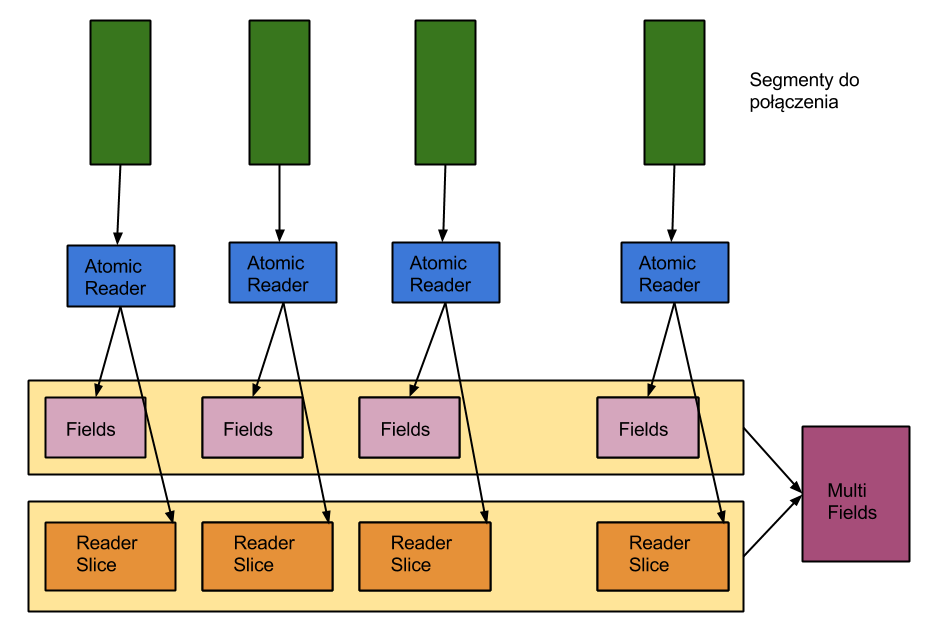
\includegraphics[scale=0.4]{pictures/LaczeniePol.png}
 \caption{Schematyczne ujęcie procesu łączenia pól z różnych segmentów. Źródło: opracowanie własne. \label{fig:fieldMerge}}
\end{figure}

\section{\texttt{MultiFields}}

\texttt{MultiFields} jest rozszerzeniem klasy \texttt{Fields}. Grupuje w sobie reprezentacje pól pochodzących z różnych segmentów i pozwala na operowanie ich zawartością tak, jakby były to pola pobrane z jednego segmentu. Jego schemat (oraz schematy klas powiązanych) przedstawia rys. \ref{multiFields}.

\begin{figure}[here]
 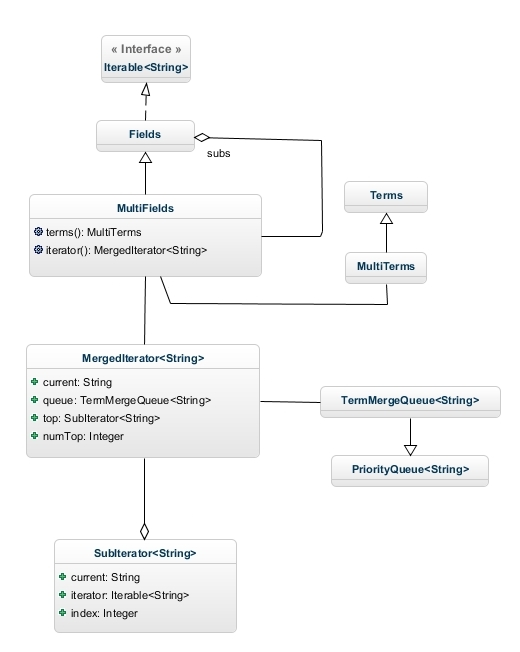
\includegraphics[scale=0.65]{pictures/MultiFields_1.jpg}
 \caption{\texttt{MultiFields} oraz klasy powiązane. Źródło: opracowanie własne.\label{multiFields}}
\end{figure}

To, że \texttt{MultiFields} jest rozszerzeniem klasy \texttt{Fields} oznacza, że posiada wszystkie jej funkcjonalności i w ich obrębie posługuje się takim samym interfejsem. Z punktu widzenia klasy zarządzającej procesem łączenia segmentów (\texttt{SegmentMergera}) zachowuje się więc dokładnie jak \texttt{Fields}. Jest to przykład dobrego podziału odpowiedzialności pomiędzy klasami i ukrywania wewnętrznej implementacji.

Z punktu widzenia algorytmu łączenia segmentów, najbardziej interesującymi metodami \texttt{MultiFields} są \texttt{MultiFields.terms(String field)}, zwracająca termy należące do pola o podanej nazwie oraz \texttt{MultiFields.iterator()}, zwracająca iterator pozwalający na przechodzenie po kolejnych nazwach pól. 

\section{\texttt{MultiFields.terms()}}

\texttt{MultiFields.terms()} zwraca instancję typu \texttt{MultiTerms}. Podobnie jak \texttt{MultiFields} agreguje pola z różnych segmentów, ale zachowuje się tak, jak \texttt{Fields} pochodzące z pojedynczego segmentu, tak \texttt{MultiTerms}  gromadzi wszystkie termy znajdujące się w danym polu. Ukrywa też to, że dla danego termu być może mamy do czynienia z kilkoma termami o takim samym tokenie, ale pochodzącymi z tego samego pola z różnych segmentów.

Schemat tworzenia instancji \texttt{MultiTerms} znajduje się na rys. \ref{fig:multiTerms}. Nietrudno dostrzec podobieństwo z algorytmem tworzenia instancji \texttt{MultiFields} (rys. \ref{fig:fieldMerge}). Instancje \texttt{Terms} są pobrane przy pomocy \texttt{Fields.terms(f)} dla \texttt{f} będącego nazwą pola. Jeśli obiekt \texttt{Terms} istnieje dla danego pola (tzn. \texttt{terms(f) != null}), podawany jest, wraz z odpowiadającym mu obiektem \texttt{ReaderSlice}, do właśnie tworzonej instancji \texttt{MultiTerms}.

\begin{figure}[here]
 \centering
 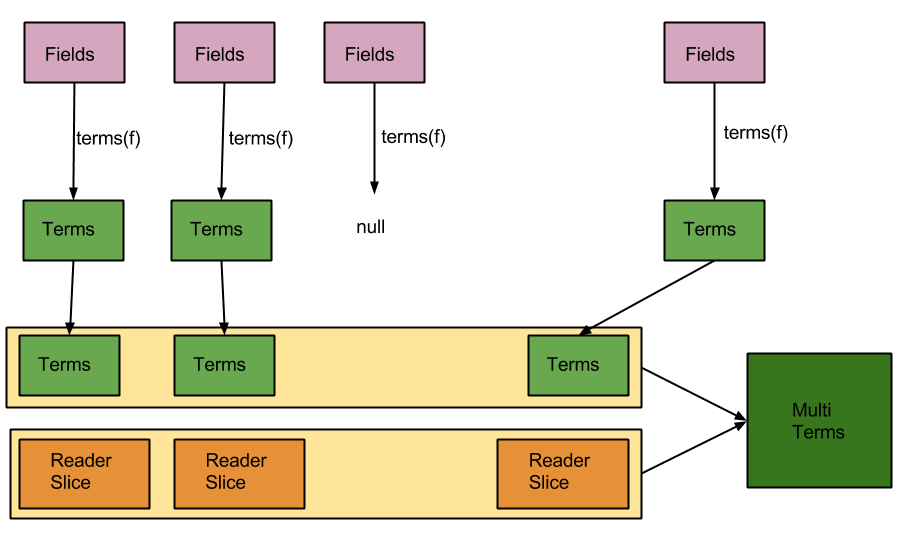
\includegraphics[scale=0.4]{pictures/MultiTerms.png}
 \caption{Schemat tworzenia instancji \texttt{MultiTerms}. Źródło: opracowanie własne. \label{fig:multiTerms}}
\end{figure}

\section{\texttt{MultiFields.iterator()}}

Jak zostało to już wspomniane, \texttt{Fields.iterator()} przechodzi po nazwach pól zgromadzonych w klasie \texttt{Fields}. Kolejne elementy zwracane przez ten iterator są uporządkowane rosnąco. \texttt{MultiFields.iterator()}, aby spełnić to wymaganie, posługuje się własną implementacją iteratora napisów -- klasą \texttt{MergedIterator}. Oto jej specyfikacja:
\begin{itemize}
 \item \texttt{MergedIterator} jest tworzony na podstawie iteratorów napisów $i_1$, $i_2$, ... $i_n$. Zwraca kolejno elementy tych iteratorów posortowane rosnąco; 
 \item jeśli dany element występuje w więcej niż jednym z iteratorów $i_1$, $i_2$, ... $i_n$, \texttt{MergedIterator} zwraca go tylko raz.
\end{itemize}
Iteratory $i_1$, $i_2$, ... $i_n$ pochodzą z instancji \texttt{Fields} zgromadzonych w \texttt{MultiFields}. \texttt{MergedIterator} wykorzystuje kolejkę priorytetową do przechowywania zagregowanych iteratorów. Porządek kolejki jest zdefiniowany przez elementy, na które w danym momencie wskazują iteratory $i_k, k \in \{1, ..., n\}$.

\section{Łączenie termów}

Łączenie termów odbywa się w metodzie \texttt{merge()} klasy \texttt{TermsConsumer}, która jako parametry przyjmuje:
\begin{itemize}
 \item \texttt{MergeState} -- pomocniczy obiekt przechowujący stan obecnego procesu łączenia segmentów. Gromadzi listę \texttt{AtomicReaderów}, strukturę z informacją o dokumentach do usunięcia, itp. Nie będziemy się nim zajmować w dalszej części pracy;
 \item \texttt{IndexOptions} -- wartość wskazująca na to, jakie informacje o termach i ich wystąpieniach zostały zaindeksowane. \texttt{IndexOptions} przyjmuje jedną z czterech wartości:
 \begin{enumerate}
  \item \texttt{DOCS\_ONLY}: oznacza, że w indeksie znajduje się tylko informacja o tym, czy dany term tam wystąpił, czy nie. Częstości występowania termu oraz pozycje wystąpień są pominięte -- co skutkuje np. tym, że zapytania frazowe nie mogą zostać na takim indeksie wykonane. Obliczanie zgodności zapytania z dokumentem zachowuje się tak, jakby każdy term występował w dokumencie dokładnie raz.
  \item \texttt{DOCS\_AND\_FREQS}: dla każdego termu zapamiętana jest informacja o jego liczbie wystąpień w dokumencie. Dzięki temu podobieństwo zapytania do dokumentu może być obliczone precyzyjniej. Zapytania frazowe oraz inne, wykorzystujące informacje o pozycjach termów, nie mogą być wykonywane.
  \item \texttt{DOCS\_AND\_FREQS\_AND\_POSITIONS}: najczęściej wykorzystywany sposób indeksowania: w indeksie pamiętane są częstości termów oraz pozycje ich wystąpień, w związku z czym możliwe jest wykonywanie wielu typów zapytań.
  \item \texttt{DOCS\_AND\_FREQS\_AND\_POSITIONS\_AND\_OFFSETS}: poza częstościami i pozycjami wystąpień termów pamiętane są informacje o dokładnym położeniu każdego termu (tzn. odległości znakowej od początku dokumentu) i jego faktycznej długości (pamiętamy o tym, że różne formy danego termu podczas analizy są sprowadzane do formy bazowej -- dlatego informacja o pierwotnej długości wystąpienia musi być dodatkowo zapamiętywana).
 \end{enumerate}
 \item \texttt{TermsEnum} -- w procesie łączenia termów będzie to instancja \texttt{MultiTermsEnum}, pobrana z obiektu \texttt{MultiTerms}.
\end{itemize}

W najprostszym przypadku -- dla opcji \texttt{DOCS\_ONLY} -- algorytm łączenia termów wygląda następująco:
\begin{enumerate}
 \item Zainicjalizuj zbiór dokumentów odwiedzonych już dla właśnie łączonego termu (\texttt{visitedDocs}).
 \item Zainicjalizuj pole \texttt{docsEnum} typu \texttt{MappingMultiDocsEnum}, o ile nie zostało to jeszcze zrobione (leniwa inicjalizacja -- właśnie łączony term jest pierwszym z termów pola).
 \item Dla każdego termu \texttt{t} dostępnego z \texttt{MultiTermsEnum} pobierz listę \texttt{docsEnumIn} dokumentów, w których term ten występuje. Lista opakowana jest w instancję klasy \texttt{MultiDocsEnum}. Dodaj dokumenty z \texttt{docsEnumIn} do \texttt{docsEnum}. Wykonaj kroki \ref{enum:begin} -- \ref{enum:end} dla \texttt{t}.
 \item \label{enum:begin} Rozpocznij zapis listy postingowej dla \texttt{t} (przy pomocy wywołania \texttt{startTerm(t)}). Jednocześnie pobierz instancję \texttt{PostingsConsumera}, która umożliwi połączenie list postingowych pochodzących z różnych segmentów.
 \item Wywołaj \texttt{PostingsConsumer.merge()}, jako parametry przekazując obiekt przechowujący stan, \texttt{DOCS\_ONLY} jako opcję indeksowania, \texttt{docsEnum} i listę odwiedzonych już dokumentów.
 \item \label{enum:end} Zakończ zapis termu (\texttt{PostingsConsumer.finishTerm()}), zapamiętaj liczbę dokumentów w połączonej liście.
\end{enumerate}

Dla pozostałych wartości parametru \texttt{IndexOptions} łączenie termów przebiega podobnie. Różni się jedynie typami struktur przechowujących referencje do list postingowych.
\begin{itemize}
 \item W przypadku \texttt{DOCS\_AND\_FREQS} korzystamy z innej instancji typu \texttt{MappingMultiDocsEnum}, \texttt{docsAndFreqsEnum}, zamiast \texttt{docsEnum}.
 \item W przypadkach \texttt{DOCS\_AND\_FREQS\_AND\_POSITIONS} i \texttt{DOCS\_AND\_FREQS\_AND\_POSITIONS\_AND\_OFFSETS} korzystamy z tej samej instancji klasy \texttt{MappingMultiDocsAndPositionsEnum}, \texttt{postingsEnum}.
\end{itemize}
Różne typy i różne instancje przechowujące dane o listach postingowych są tutaj potrzebne, ponieważ w ramach jednego procesu łączenia segmentów możemy mieć do czynienia z różnymi opcjami indeksowania pól (jak już wspomniano, opcje indeksowania pól są całkowicie od siebie niezależne, nawet dla pól występujących w tym samym segmencie).

\section{Łączenie list postingowych}

Łączenie list postingowych jest zaimplementowane w metodzie \texttt{merge()} klasy \texttt{PostingsConsumer}. Metoda ta przyjmuje następujące parametry:
\begin{itemize}
 \item \texttt{MergeState}: tutaj niepotrzebny, nigdzie nie używany. Prawdopodobnie jest to pozostałość po starej implementacji i zostanie usunięta w najbliższym czasie.
 \item \texttt{IndexOptions}: podobnie, jak w przypadku łączenia termów, dokładny algorytm zależy od wybranej opcji indeksowania.
 \item \texttt{DocsEnum}: reprezentacja list dokumentów, które mają być połączone. Obecny kodek wykorzystuje \texttt{MappingMultiDocsEnum} lub \texttt{MappingMultiDocsAndPositionsEnum}, w zależności od opcji indeksowania (i instancji przekazanej tutaj z \texttt{TermsConsumer.merge()}). 
 \item \texttt{FixedBitSet}: zbiór bitowy reprezentujący odwiedzone już dokumenty.
\end{itemize}

Podobnie, jak w \texttt{TermsConsumer.merge()} opcje indeksowania wpływają na algorytm łączenia list. W najprostszym przypadku (dla \texttt{IndexOptions.DOCS\_ONLY} algorytm ten ma następujący przebieg:
\begin{enumerate}
 \item \label{jeden} Pobierz kolejny posting z listy (z \texttt{DocsEnum}) do zmiennej \texttt{doc}. Jeśli otrzymaną wartością jest \texttt{NO\_MORE\_DOCS}, zakończ algorytm. W przeciwnym wypadku przejdź do kroku \ref{dwa}
 \item \label{dwa} Zaznacz \texttt{doc} jako odwiedzony (skorzystaj z dostarczonej instancji \texttt{FixedBitSet}).
 \item \label{trzy} Rozpocznij zapis postingu. Wpisz wartość \texttt{doc}.
 \item Zakończ zapis postingu.
 \item Przejdź do kroku \ref{jeden}.
\end{enumerate}

W przypadku innych opcji indeksowania do powyższego algorytmu wprowadza się kilka zmian.
\begin{itemize}
 \item Dla opcji \texttt{DOCS\_AND\_FREQS}, poza pobraniem postingu z listy \texttt{DocEnum} w kroku \ref{jeden}, odczytuje się także częstość występowania termu w dokumencie, \texttt{docFreq}, która później zapisywana jest wraz z postingiem w kroku \ref{trzy}.
 \item Dla opcji \texttt{DOCS\_AND\_FREQS\_AND\_POSITIONS} dodatkowo odczytywane są (i później zapisywane do listy wynikowej) pozycje wystąpień termu w dokumencie oraz ewentualne \emph{payloads}, a dla \texttt{DOCS\_AND\_FREQS\_AND\_POSITIONS\_AND\_OFFSETS} -- również ich odległości znakowe od początku dokumentu i długości.
\end{itemize}

\section{Rozszerzenia klasy \texttt{DocsEnum} używane w procesie łączenia postingów}

\texttt{DocsEnum} jest abstrakcją pozwalającą pobierać kolejne elementy list postingowych. Jej interfejs zawiera jedynie metody zwracające numer dokumentu obecnie wskazywanego przez iterator, jego częstość oraz pozwalające na przejście do kolejnych dokumentu. Dodatkowe funkcjonalności są implementowane przez jej liczne rozszerzenia (np. wspomniany już \texttt{DocsAndPostitionsEnum}). W algorytmie łączenia list postingowych wykorzystywane są cztery z nich: \texttt{MultiDocsEnum}, \texttt{MappingMultiDocsEnum} oraz odpowiadające im \texttt{MultiDocsAndPositionsEnum} i \texttt{MappingMultiDocsAndPositionsEnum}. Przyjrzymy się im dokładniej.

Podczas łączenia termów (w metodzie \texttt{TermsConsumer.merge()}) z iteratora termów (konkretniej: z instancji \texttt{MultiTermsEnum}) pobierany jest obiekt \texttt{MultiDocsEnum}. Zawiera on informacje o listach postingowych dla danego termu pochodzących z łączonych segmentów oraz odpowiadające im wskaźniki na dany segment (w postaci obiektów \textt{ReaderSlice}). 
